\documentclass[oneside,12pt]{wipb}

\katedra{Oprogramowania}
\typpracy{inżynierska}
%typpracy{magisterska}
\temat{Aplikacja internetowa do obsługi system gdt w technologii Python/Django.}
\autor{Mateusz Pernal}
\promotor{dr inż. Krzysztof Jurczuk}
\indeks{101420}
\studia{stacjonarne}
\rokakademicki{2019/2020}
\profil{studia I stopnia}
\kierunekstudiow{informatyka}
\specjalnosc{Brak}
\zakres{1. Zapoznanie z systemem GDT \newline 2. Analiza wymagań aplikacji\newline 3. Projekt i implementacja aplikacji \newline 4. Testy oraz wdrożenie aplikacji.}

\hypersetup{
pdfauthor={Mateusz Pernal},
pdftitle={Praca inżynierska},
pdfsubject={Aplikacja internetowa do obsługi systemu GDT w technologii Python/Django},
pdfkeywords={praca inżynierska słowa klucz },
pdfpagemode=UseNone,
linkcolor=black,
citecolor=black,
urlcolor=black
} 

\setlength{\epigraphwidth}{1\textwidth}

\begin{document}

\maketitle

\chapter*{\centering{\vspace{1in}Summary}}
\addcontentsline{toc}{chapter}{Streszczenie}
 
\epigraphhead[40]{
Subject of diploma thesis: Internet application to support the GDT system in Python/Django technology.}

The aim of this thesis was to design, implement and introduce a web application to support GDT (\textit{Global Decision Trees}) system using Python and Django technologies. In the basic version, GDT is a console program for creating decision trees. The requirement of the project was to create a web application allowing to create, delegate and manage the tasks launched by using the GDT system. The developed tool will also provide graphical representation of the obtained results.

The thesis consists of four chapters. First chapter describes the problem and presents the decision trees. It also shows the most popular existing solutions. Second chapter contains an analysis of project requirements and a overview of the technologies that have been used. Third chapter is intended to present the system architecture. It illustrates most important mechanisms and solutions created for the application. It also shows the database schema with a short description of tables. Fourth chapter contains a overview of particular views of the application, but also an example how to use them. In addition, it presents the results of load and manual tests.


%\biblioteka{}

\pagestyle{plain}

\setcounter{tocdepth}{1}
\tableofcontents

\chapter*{Wprowadzenie}
\addcontentsline{toc}{chapter}{Wprowadzenie}
Proces myślowy człowieka jest w dużej mierze oparty o~pewien schemat podejmowania decyzji. Podejmowane decyzje mają kluczowy wpływ na jego aktualne życie i~przyszłość. Wybór najbardziej optymalnego rozwiązania danego problemu wymaga dokładnej analizy dostępnych informacji. Posiadając wystarczającą ilość danych możemy wykorzystać różne algorytmy, które mogą pomóc podjąć właściwy wybór. Mechanizm podejmowania decyzji bezpośrednio dotyczy nie tylko człowieka, a~wszystkiego co znajduje się w~jego otoczeniu. 

Szybki rozwój technologi w XX i XXI wieku prowadzi do produkowania i~gromadzenia coraz większej ilości informacji. Firmy starają się wyciągnąć ze zgromadzonych danych możliwe jak najlepsze wnioski. Poddając analizie tak duże zbiory informacji wymagane jest zastosowanie narzędzi uproszczających i~przyśpieszających uzyskanie wyników. Prowadzi to do tworzenia algorytmów oraz mechanizmów zarówno obróbki danych, jak i ich analizy w~celu osiągnięcia zadowalających rezultatów. W przeciągu ostatnich kilkunastu lat entuzjazm związany z~technikami komputerowymi wzrósł gwałtownie i~zdominował przemysł. Uczenie maszynowe wraz z~analizą danych stanowi bardzo ważny element rozwiązań produkowanych przez firmy. Wspomaga takie technologie, jak rozpoznawanie mowy, pisma czy też autonomiczne samochody i~roboty sprzątające. Wszystkie te rozwiązania wymagają przetwarzania ogromnych ilości informacji, w jak najkrótszym czasie oraz podjęcie wystarczająco dobrej decyzji.

W pracy tej rozwijany będzie system do uczenia maszynowego GDT (\textit{Global Decision trees})\cite{sgdt_1} tworzony przez pracowników Politechniki Białostockiej. System ten służy do generowania drzew decyzyjnych na podstawie zbioru uczącego. Drzewa generowane są z~wykorzystaniem algorytmów ewolucyjnych (metoda alternatywna do algorytmów zachłannych typu \textit{top-down}). Aplikacja GDT jest programem konsolowym. W celu ułatwienia dostępu do platformy GDT większemu gronu użytkowników w niniejszej pracy zostanie zaprojektowana, zaimplementowana oraz wdrożona aplikacja do obsługi systemu GDT z~poziomu przeglądarki internetowej.  

%Rozwiązania z dziedziny uczenia maszynowego również są tworzone przez pracowników Politechniki Białostockiej. Autorski system GDT opiera się na generowaniu drzew decyzyjnych dla zbiorów z danymi wejściowymi. Mechanizm odpowiadający za obliczenie rezultatów wykorzystuje w swoim działaniu algorytmy genetyczne. Obsługa systemu przebiega po przez konsolę systemową, co wiąże się ze znajomością chodź podstawowych komend. W celu ułatwienia dostępu do platformy GDT istnieje potrzeba zaprojektowania interfejsu graficznego opartego o technologie webowe.  

\section*{Cel pracy}
Celem pracy jest stworzenie aplikacji webowej umożliwiającej obsługę systemu GDT. Aplikacja ta będzie umożliwiać tworzenie, zlecanie oraz zarządzanie zadaniami uruchamianymi przy pomocy systemu. Podczas tworzenia zadań użytkownik powinien móc ustawić opcje dotyczące, np. wybranego algorytmu oraz jego parametrów. Aplikacja powinna także udostępniać opcje związane z wyświetleniem drzewa wynikowego w postaci graficznej, jego eksport do pliku oraz wgląd do pozostałych wyników uruchomianego algorytmu.
\section*{Zakres pracy}
Zakres pracy obejmuje: 

\begin{itemize}
\item Zapoznanie z systemem GDT,
\item Analiza wymagań aplikacji,
\item Projekt i implementacja aplikacji, 
\item Testy oraz wdrożenie aplikacji.
\end{itemize}


\section*{Organizacja pracy}
Praca została podzielona na cztery główne części. Pierwsze dwa rozdziały zawierają przedstawienie problemu, analizę wymagań i~wykorzystane technologie. W dalszej części pracy została omówiona architektura aplikacji wraz z zastosowanymi rozwiązaniami. Natomiast prezentacja stworzonej aplikacji oraz opis testów został przedstawiony w~rozdziale 4.

Rozdział 1 zawiera opis mechanizmu tworzenia drzew decyzyjnych. Przedstawia również zagadnienia związane z systemem GDT. Porusza też temat podobnych aplikacji dostępnych w~internecie.

Rozdział 2 przedstawia analizę wymagań funkcjonalnych i~niefunkcjonalnych tworzonej aplikacji. Został w nim zamieszczony diagram przypadków użycia wraz z~ich opisem oraz diagram czynności. Następnie zaprezentowany został schemat rozwiązania. Rozdział kończy przedstawienie użytych technologi podczas tworzenia aplikacji.

Rozdział 3 przedstawia architekturę tworzonej aplikacji. Prezentuje najważniejsze mechanizmy oraz rozwiązania stworzone na potrzeby aplikacji. Przedstawia także schemat bazy danych wraz z krótkim opisem najważniejszych tabel.

Rozdział 4 przedstawia stworzoną aplikację. Zawiera on opis poszczególnych widoków aplikacji, ale także przykładowy sposób ich użycia. Ponadto przedstawia wyniki testów obciążeniowych i manualnych przeprowadzonych przez studentów Wydziału Informatyki Politechniki Białostockiej.
\chapter{Przedstawienie problemu}

\section{Drzewa decyzyjne}

Podejmowanie decyzji jest procesem myślowym, który od początku istnienia ludzkości stwarza pewne trudności, a polega on na wybraniu najlepszego rozwiązania z dostępnych. Wpływ na optymalną decyzję mają informacje, które zostaną poddane analizie, ale także sama metoda analizy. Racjonalny wybór może być wspomagany różnymi algorytmami, czy też wizualną reprezentacją możliwych decyzji w postaci diagramu. Sam diagram może przybrać formę graficzną drzewa decyzyjnego.

Podstawowymi elementami drzewa są korzeń, gałęzie, węzły oraz liście. Korzeniem jest decyzja od którego rozpoczyna się budowa całej struktury, której poszczególne węzły, odpowiadające za sprawdzenie pewnego warunku, są połączone gałęziami.\cite{misc_1}  Liście są krańcowymi wierzchołkami drzewa i określają wybraną decyzje. Podczas próby określenia decyzji, należy poddać klasyfikacji posiadane dane. Aby to zrobić konieczne jest przejście całego drzewa od samego korzenia do wynikowego liścia. Rezultatem takiej operacji będzie klasa definiująca decyzję.

\section{Uczenie maszynowe}
W otaczającym nas świecie ilość informacji produkowanych przez otoczenie oraz zbieranych przez firmy czy instytucje nadal przewyższa ilość danych, które można przeanalizować z użyciem obecnych zasobów. Chcąc choć w jakimś stopniu poddać analizie duże ilości danych, aby na ich podstawie wyciągnąć wnioski używa się licznych rozwiązań technologicznych. Dzięki zastosowaniu różnych algorytmów przetwarzania danych, klasyfikacji oraz predykcji istnieje możliwość umożliwienia uczenia się programowi komputerowemu. Kierunek nauki, który zajmuje się tą dziedziną nazywamy uczeniem maszynowym. W ciągu ostatnich dziesięciu lat entuzjazm związany z wykorzystywaniem tej technologi wzrósł gwałtownie i w dużej mierze 
zdominował przemysł, ale również przyczynił się do jej rozwoju.\cite{book_1} Uczenie maszynowe stanowi trzon wielu usług, serwisów i aplikacji. Pod względem technologicznym odpowiada za wyniki wyszukiwania w przeglądarkach, za rozpoznawanie mowy przez nasze telefony, ale także jest odpowiedzialne za prowadzenie autonomicznych samochodów.

\section{Drzewa decyzyjne w technikach uczenia maszynowego}

Drzewa decyzyjne stanowią jedne z bardziej wszechstronnych algorytmów w  dziedzinie uczenia maszynowego. Z jednej strony mogą być wykorzystywane w zadaniach z zakresu klasyfikacji, a z drugiej strony również odgrywają ważną rolę w regresji.\cite{book_1} Z ich pomocą możemy uzyskać potężne modele i narzędzia zdolne do uczenia się ze złożonych zbiorów danych. Dodatkowym atutem drzew jest możliwość wizualnego przedstawienia rozwiązania, które będzie zrozumiałe dla osób nie mających do czynienia z uczeniem maszynowym lub ze statystyką. Z racji wzrostu popularności tej technologi zwiększyły się nakłady pracy naukowej w celu osiągnięcia coraz to lepszych i bardziej optymalnych algorytmów pod względem wydajnościowym. 

\subsection{System GDT}
Pracownicy Politechniki Białostockiej również mają wkład w budowę takich rozwiązań. Autorski system GDT (\textit{Global Decision Trees}), który jest wykorzystywany w aplikacji inżynierskiej, służy do generowania modelu drzewa decyzyjnego na podstawie zbiorów wejściowych. Ten system jest zaimplementowany w języku c++ oraz jest skompilowany do pliku wykonywalnego, aby umożliwić jego uruchomianie z poziomu konsoli systemu operacyjnego. Całe rozwiązanie jest unikalne i nie ma takiego drugiego identycznego, a głównym założeniem jest wykorzystanie algorytmów genetycznych. Z ich pomocą przestrzeń rozwiązań danego problemu jest większa niż w klasycznym podejściu, co skutkuje możliwością osiągnięcia dokładniejszych i lepszych wyników. Metody pracy algorytmów genetycznych w dużej mierze odwzorowują działania samej natury.\cite{book_2} Podczas definiowania pracy algorytmu należy podać takie parametry jak wielkość populacji, prawdopodobieństwo mutacji czy też krzyżowania się danych osobników. Wartości tych parametrów i innych są określane w pliku konfiguracyjnym opartym o strukturę XML, który jest zarazem plikiem wejściowym do aplikacji GDT. System oprócz tego pliku wykorzystuje pliki z konkretnymi rozszerzeniami:
\begin{itemize}
	\item *.data - plik zawierający dane treningowe, 
	\item *.test - plik zawierajacy dane testowymi,
	\item *.names - plik określających nazwy klas oraz rodzaj zmiennych.
\end{itemize}
Na podstawie tych danych aplikacja GDT może stworzyć model drzewa decyzyjnego, którego przedstawienie jest zapisywane w pliku tekstowym. 

\section{Istniejące rozwiązania}
\chapter[Inny tytu� do spisu tre�i]{Inne przyk�ady}
\section{Cytowania}
Literature cytujemy przez $\backslash cite\{nazwa1,nazwa2\}$ przyk�adowo $\backslash cite{NagraTC02}$ da w efekcie \cite{NagraTC02} lub $\backslash cite\{NagraTC02,iso9126\}$ - \cite{NagraTC02,iso9126}.
\section{Wypunktowania}
Wypunktowanie stosujemy 
\begin{verbatim}
    \begin{enumerate}
    \item pierwsze
    \item drugie
    \end{enumerate}
\end{verbatim}
co daje efekt jako:
    \begin{enumerate}
    \item pierwsze
    \item drugie
    \end{enumerate}
lub te� jako
\begin{verbatim}
    \begin{itemize}
    \item jeden
    \item dwa
    \end{itemize}
\end{verbatim}
co daje efekt jako:
    \begin{itemize}
    \item jeden
    \item dwa
    \end{itemize}
\subsection{Wypunktowania mieszane}
\begin{verbatim}
\begin{enumerate}
    \item 1
    \begin{itemize}
        \item 1.1
        \item 1.2
    \end{itemize}
    \item 2
    \begin{itemize}
        \item 2.1
        \item 2.2
\end{itemize}
\end{enumerate}
\end{verbatim}
efekt ko�cowy
\begin{enumerate}
    \item 1
    \begin{itemize}
        \item 1.1
        \item 1.2
    \end{itemize}
    \item 2
    \begin{itemize}
        \item 2.1
        \item 2.2
\end{itemize}
\end{enumerate}
\section{Tabele}
Tabele wstawiamy przez
\begin{verbatim}
\begin{table}[t]
\centering
\begin{tabular}{|ccc|}%rodzaj kolumn
\hline
1 kolumna & 2 kolumna & 3 kolumna \\
\hline
\end{tabular}
\caption{Opis tabeli}
\label{tab:p1}%referencja
\end{table}
\end{verbatim}
\begin{table}[t]
\centering
\begin{tabular}{|ccc|}%rodzaj kolumn
\hline
1 kolumna & 2 kolumna & 3 kolumna \\
\hline
\end{tabular}
\caption{Opis tabeli}
\label{tab:p1}%referencja
\end{table}
Do tebeli odwo�ujemy si� przez

\chapter{Architektura rozwiązania}
\section{Architektura aplikacji}
Struktura aplikacji jest oparta na podziale wynikającym z wykorzystania frameworka Django. Zgodnie z tym założeniem projekt dzieli się na poszczególne moduły, które w rozumieniu platformy nazywane są paczkami.  W aplikacji można wyróżnić cztery podstawowe elementy kolejno odpowiadające za zarządzanie eksperymentami i użytkownikami, interfejs graficzny oraz aplikacja zbierająca wszystko w całość. Schemat modułów jest przedstawiony na Rys. \ref{rys4_packages}. 

Aplikacja jest zaimplementowana zgodnie ze stylem architektonicznym REST (\textit{Representational State Transfer}). Architektura ta jest bardzo popularna przy tworzeniu aplikacji internetowych ze względu na swoją lekkość oraz prostotę. Do komunikacji pomiędzy widokami aplikacji, a logiką biznesową znajdującą się na serwerze, wykorzystywany jest protokół http. W tym celu do każdej poszczególnej funkcjonalności działającej w projekcie musiał zostać wystawiony endpoint. Zbiór wszystkich wystawionych serwisów przyjmuje nazwę API \textit{(Application Programming Interface)}. Taki rodzaj rozwiązania zapewnia jasny podział na poszczególne warstwy, które są od siebie niezależne. Dzięki temu część serwerowa aplikacji może działać nie ingerując w część interfejsu graficznego. Mapowaniem poszczególnych modułów aplikacji na endpointy zajmuje się główna aplikacja \enquote{decisionTree}. 


Obok plików aplikacji można wyróżnić folder \enquote{users} zawierający foldery użytkowników. Nazwy tych katalgów są tworzone na bazie loginu. Każdy użytkownik może wgrywać dowolną ilość plików o rozszerzeniach \enquote{*.xml}, \enquote{*.data}, \enquote{*.test} oraz \enquote{*.names} do swojego folderu. Podczas tworzenia nowego eksperymentu tworzony jest dla niego katalog o nazwie składającej się z pola  \enquote{id} i \enquote{name}. Tam są przechowywane wszystkie pliki  związane z doświadczeniem. Użytkownik ma możliwość pobrania całego folderu z plikami eksperymentu w postaci archiwum o rozszerzeniu  \enquote{*.zip}. Dodatkowo w aplikacji jest dostępna opcja zarządzania katalogiem głównym użytkownika. Udostępnione są opcje do zmiany nazwy, usunięcia czy też pobrania pliku. 

\begin{figure}[htb]
	\centering
	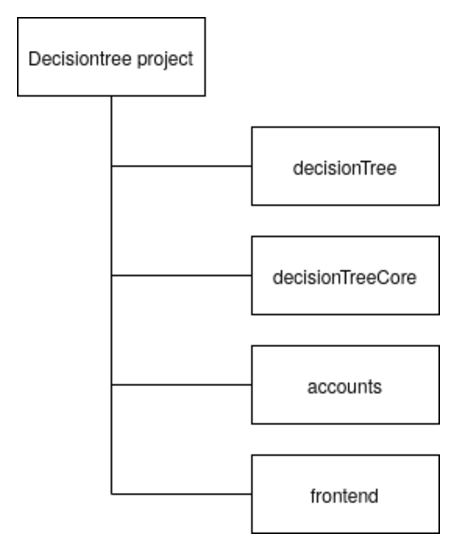
\includegraphics[height=8cm]{grafika/packages.eps}
	\caption{Podział projektu na moduły, źródło: opracowanie własne}
	\label{rys4_packages}
\end{figure}
%\subsection{Generowanie postępu}
Użytkownik uruchamiając nowy eksperyment, powinien widzieć jego postęp, jak i średni czas, który pozostał do końca. Zostało to rozwiązane w aplikacji po przez tabelę w bazie pośredniczącą wymianie informacji o progresie doświadczania. Program uruchomiony w robotniku Celery, wypisuje informacje na standardowe wyjście (stdin). W tych danych znajduje się numer iteracji wykonanej oraz średni jej czas. Stosując połączenie za pośrednictwem PIPE, robotnik może przeanalizować te informacje. W celu ograniczenia obciążenia co dziesiąta linia jest poddawana analizie. Na podstawie zawartych tam danych oraz ilości uruchomień algorytmu uzyskanej z pliku konfiguracyjnego można wyliczyć średni czas pozostały do końca obliczeń. Natomiast pasek postępu zostaje wyznaczony poprzez określenie numeru ostatniej iteracji i stwierdzeniu ile wykonań algorytmu jeszcze pozostało. 

%\subsection{Autoryzacja użytkownika}
Autoryzacja użytkowników jest nieodłącznym elementem aplikacji internetowej. W tym celu został wykorzystany mechanizm tokenów. Taki token jest przyznawany dla użytkownika po zalogowaniu lub samej rejestracji. Umożliwia on autoryzowany dostęp do strony internetowej i jest przekazywany w każdym zapytaniu. Po stronie wizualnej aplikacji jest przechowywany w \textit{local storage} przeglądarki internetowej. Każdy token posiada swój czas aktywności, a po jego wygaśnięciu lub przy dowolnym problemie z jego uwierzytelnieniem użytkownik zostanie przekierowany na stronę główną. 

\section{Przechowywanie danych}
W celu przechowywania wszelkich informacji została wykorzystana relacyjna baza danych PostgresSQL. Platforma ta jest postawiona na oddzielnym kontenerze w celu uzyskania większej stabilności i nie zależności od głównego modułu aplikacji. Schemat struktury wszystkich tabel został przedstawiony na Rys. \ref{rys5_database_schema}. Większość tabel wynika z samego zastosowania frameworka Django i DjangoRestFramework. Wykorzystując gotowe rozwiązana zostały zapewnione takie modele jak \enquote{auth\_user} odpowiadający za zapisywanie informacji o użytkownikach, czy też \enquote{authtoken\_token} mająca na celu przetrzymywanie tokenów autoryzacji. Do całej struktury zostały dodane dodatkowe tabele:
\begin{itemize}
	\item \enquote{decisionTreeCore\_experiment} przetrzymująca dane o eksperymentach,  
	\item \enquote{decisionTreeCore\_permissions} zawierająca informacje o prawach dostępowych do eksperymentu,
	\item \enquote{decisionTreeCore\_progress} składa się z pól określających postęp wykonywania doświadczenia.
\end{itemize}
\begin{figure}[htb]
	\centering
	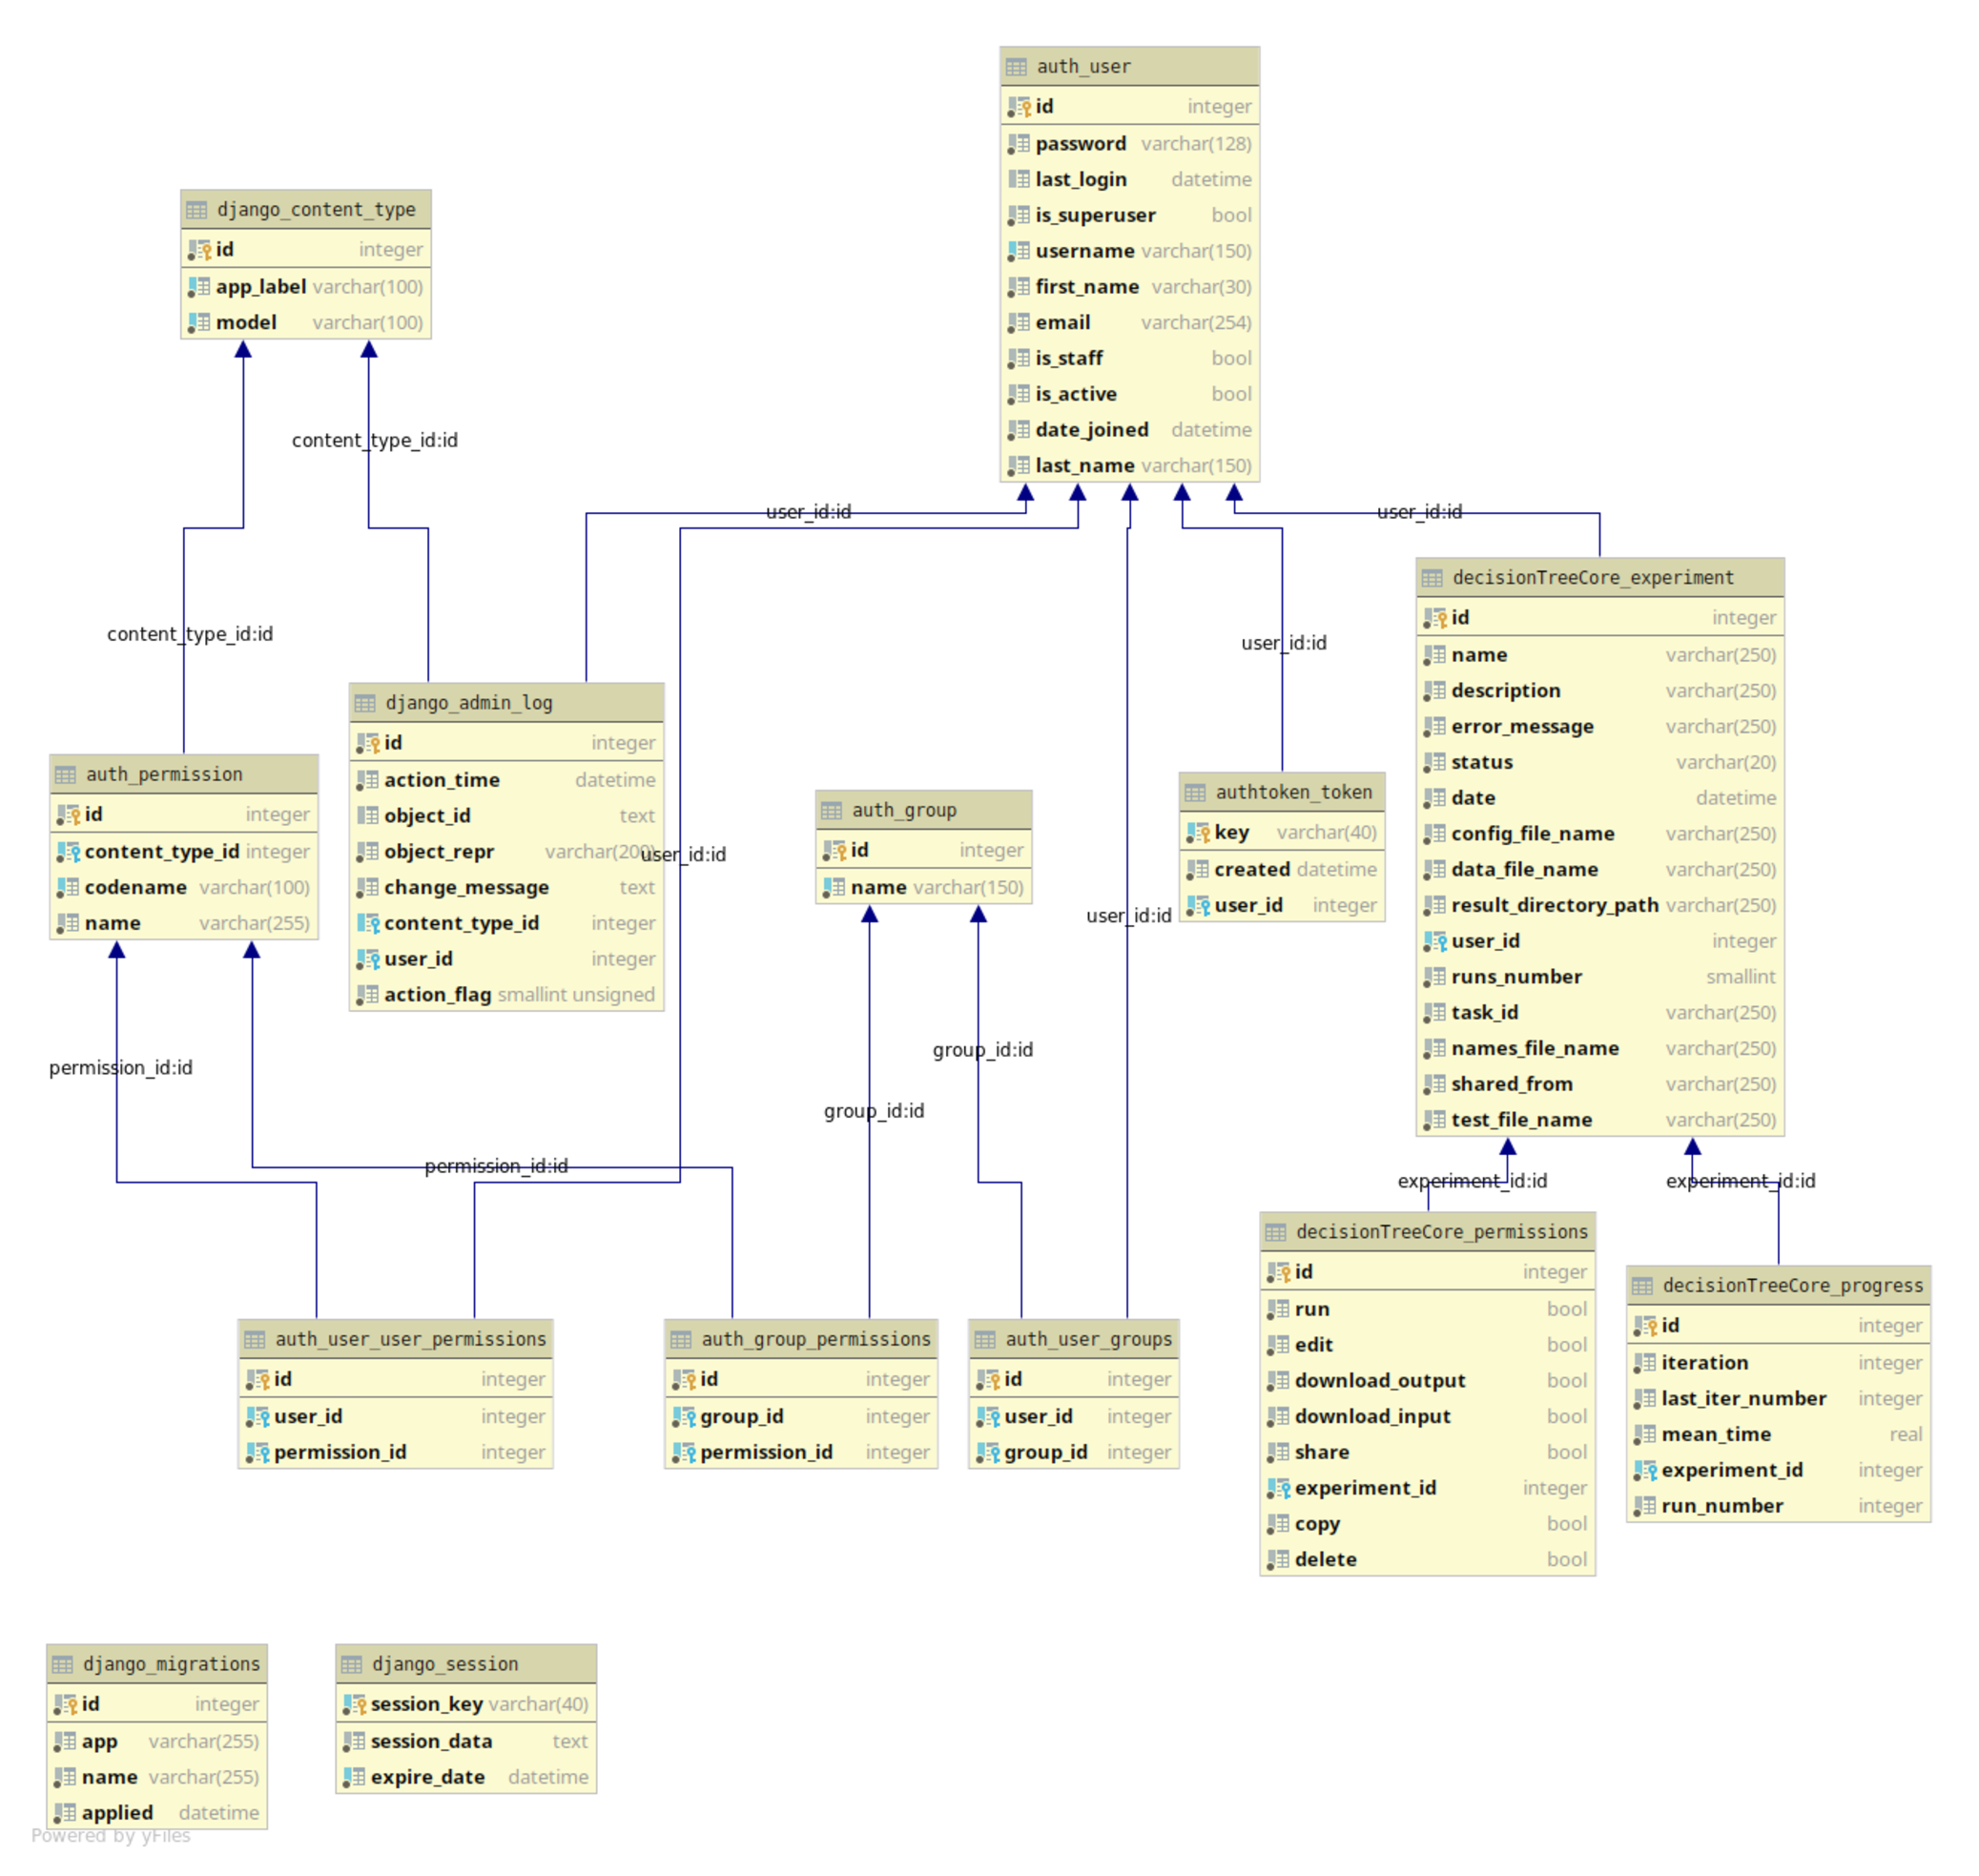
\includegraphics[angle=270, width=16cm]{grafika/database_schema.eps}
	\caption{Schemat bazy danych, źródło: opracowanie własne}
	\label{rys5_database_schema}
\end{figure}
Relacja pomiędzy nowo stworzonymi tabelami, a użytkownikiem została przedstawiona na Rys. \ref{rys6_database_schema}. Tabela \enquote{decisionTreeCore\_experiment} zawiera informacje o pojedynczym eksperymencie użytkownika, w Tab.\ref{tabela_1_schema_experiment} znajduje się opis jej pól. W celu śledzenia postępu danego doświadczenia została stworzona tabela \enquote{decisionTreeCore\_progress}. Poszczególne pola zostały rozpisane w Tab.\ref{tabela_2_schema_progress}. Dane do tej tabeli są wpisywane prosto z robotnika Celery, przy czym brana jest pod uwagę tylko co dziesiąta iteracja systemu GDT. Ostatnią dodaną tabelą na potrzeby aplikacji jest tabela  \enquote{decisionTreeCore\_permissions} określająca zakres uprawnień do danego eksperymentu. Schemat pól encji został rozpisany w Tab.\ref{tabela_3_schema_permissions}. Prawa dostępowe do doświadczenia są definiowane przez użytkownika przed samym udostępnieniem. Kolejny właściciel nie może rozszerzyć uprawnień uprzednio zablokowanych.  


\begin{table}[htb]
	\centering
	\begin{tabular}{|c|c|p{9cm}|}
		\hline
		\textbf{Nazwa pola} & \textbf{Typ} & \textbf{Opis} \\\hline
		id & integer & Klucz główny tabeli \\\hline
		name & varchar(50) & Nazwa eksperymentu\\\hline
		description & varchar(250) & Opis eksperymentu\\\hline
		error\_message & varchar(250) & Wiadomość o błędzie, który wystąpił podczas uruchomienia eksperyment\\\hline
		status & varchar(15) & Pole określające w jakim statusie znajduje się eksperyment. Możliwe wartości to: \enquote{Created}, \enquote{In queue}, \enquote{Running}, \enquote{Finished}, \enquote{Error}. Zmiana statusów następuje w trakcie przechodzenia eksperymentu przez kolejne etapy\\\hline
		data & datetime & Data stworzenia eksperymentu przez użytkownika\\\hline
		config\_file\_name & varchar(50) & Nazwa pliku konfiguracyjnego użytego w eksperymencie\\\hline
		data\_file\_name & varchar(50) & Nazwa pliku zawierającego zbiór uczący \\\hline
		test\_file\_name & varchar(50) & Nazwa pliku zawierającego zbiór testowy \\\hline
		names\_file\_name & varchar(50) & Nazwa pliku określającego nazwy klas oraz rodzaj zmiennych \\\hline
		result\_directory\_path & varchar(50) & Ścieżka do folderu z wynikami eksperymentu\\\hline
		user\_id & integer & ID użytkownika, który jest właścicielem eksperymentu \\\hline
		runs\_number & smallint & Pole określające ile przebiegów algorytmu ma się odbyć podczas uruchomienia eksperymentu w systemie GDT. Pełni ważną rolę przy tworzeniu paska postępu oraz określeniu liczby wyświetlanych drzew\\\hline
		task\_id & varchar(250) & Zawiera id zadania, które trafiło do robotnika Celery. Umożliwia zarządzanie danym zadaniem np. usunięcie z kolejki, lub anulowanie w trakcie trwania\\\hline
		shared\_from & varchar(250) & Pole pełni rolę zapisu informacji o poprzednich właścicielach. W wartością pola są nazwy użytkowników. Podczas kolejnych udostępnień do pola są dodawane po przecinku następne loginy  \\\hline
	\end{tabular}
	\caption[Opis pól encji \enquote{decisionTreeCore\_experiment}]{ Opis pól encji \enquote{decisionTreeCore\_experiment}}
	\label{tabela_1_schema_experiment}
\end{table}

\begin{table}[htb]
	\centering
	\begin{tabular}{|c|c|p{9cm}|}
		\hline
		\textbf{Nazwa pola} & \textbf{Typ} & \textbf{Opis} \\\hline
		id & integer & Klucz główny tabeli \\\hline
		iteration & integer & Liczba iteracji eksperymentu\\\hline
		last\_iter\_number & integer & Numer ostatniej iteracji\\\hline
		mean\_time & real & Wiadomość o błędzie, który wystąpił podczas uruchomienia eksperyment\\\hline
		experiment\_id & integer & Numer id eksperymentu, do którego jest przypisany postęp \\\hline
		run\_number & integer & Numer określający, które uruchomienie algorytmu właśnie trwa\\\hline
		
	\end{tabular}
	\caption[Opis pól encji \enquote{decisionTreeCore\_progress}]{ Opis pól encji \enquote{decisionTreeCore\_progress}}
	\label{tabela_2_schema_progress}
\end{table}

\begin{table}[htb]
	\centering
	\begin{tabular}{|c|c|p{9cm}|}
		\hline
		\textbf{Nazwa pola} & \textbf{Typ} & \textbf{Opis} \\\hline
		id & integer & Klucz główny tabeli \\\hline
		run & bool & Prawo do uruchamiania eksperymentu\\\hline
		edit & bool & Prawo do edycji\\\hline
		download\_out & bool & Prawo dające możliwość pobierania plików wyjściowych\\\hline
		download\_in & bool & Prawo dające możliwość pobierania plików wejściowych\\\hline
		share & bool & Pozwolenie do dalszego udostępniania eksperymentu\\\hline
		copy & bool & Prawo do tworzenia kopii\\\hline
		delete & bool & Prawo do usunięcia eksperymentu\\\hline
		experiment\_id & integer & Numer id eksperymentu, do którego są przypisane prawa dostępowe\\\hline
		
	\end{tabular}
	\caption[Opis pól encji \enquote{decisionTreeCore\_experiment}]{ Opis pól encji \enquote{decisionTreeCore\_permissions}}
	\label{tabela_3_schema_permissions}
\end{table}

 
\begin{figure}[htb]
	\centering
	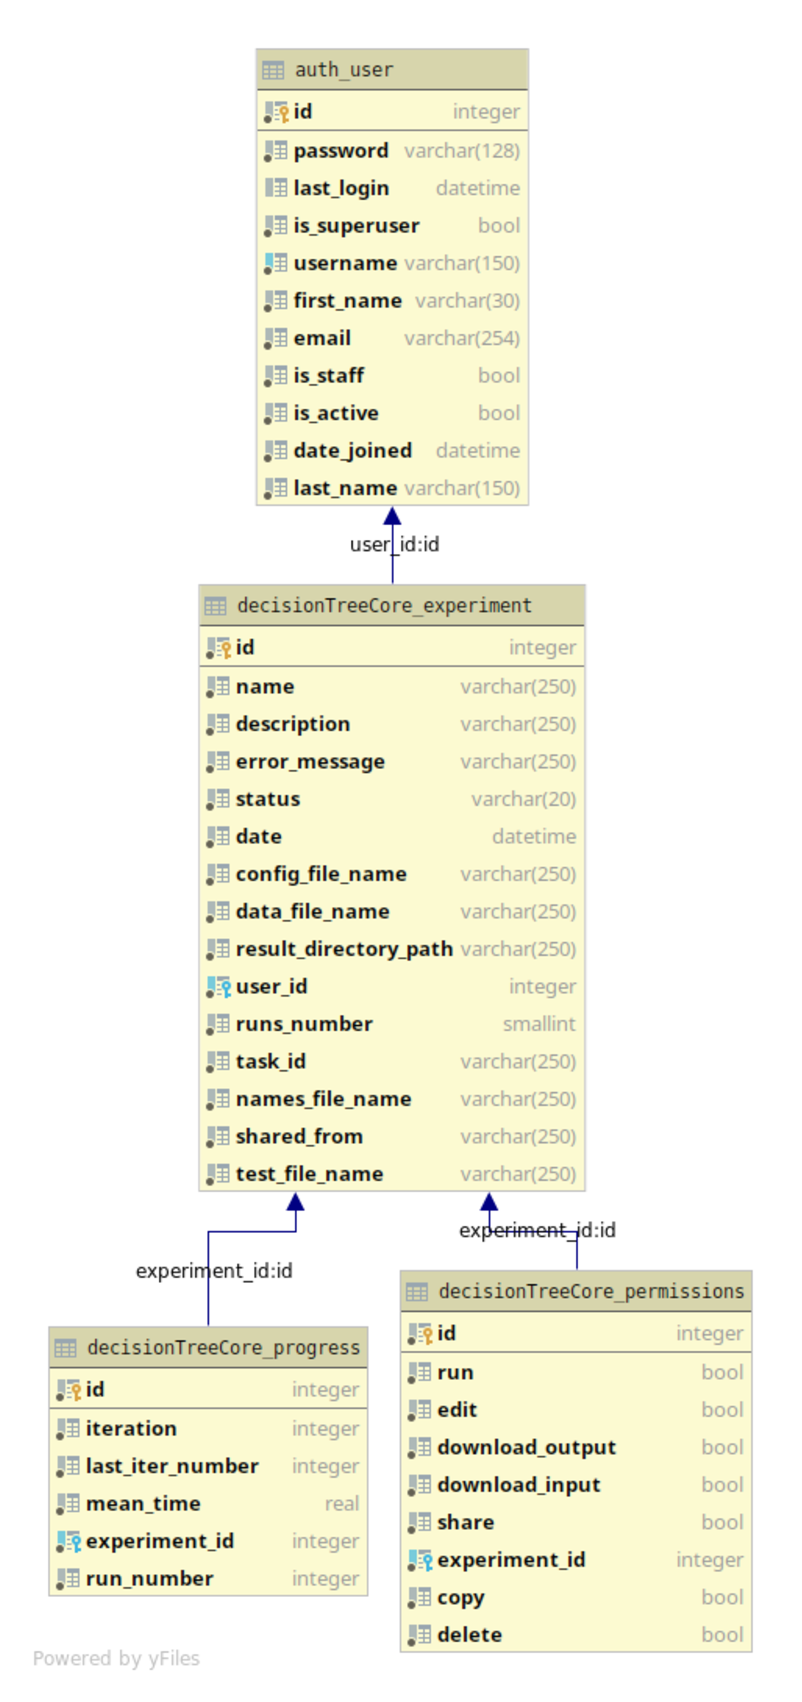
\includegraphics[height=16cm]{grafika/database_schema_2.eps}
	\caption{Schemat tabel dodatkowych, źródło: opracowanie własne}
	\label{rys6_database_schema}
\end{figure}


\subsection{Mechanizm kontroli wersji eksperymentu}
Użytkownik robiąc doświadczenie będzie chciał otrzymać jak najlepsze wyniki. W tym celu dość często będzie zmieniać parametry w pliku konfiguracyjnym. Innym przypadkiem wymagającym częstego ponownego uruchamiania eksperymentu może być zmiana plików z danymi wejściowymi. Oba ta przypadki wymagają ingerencji w plikach doświadczenia co powoduje problem, z traceniem poprzednich danych. Rozwiązaniem tej kwestii może być na przykład tworzeni kopi eksperymentu za każdym razem, gdy następuje zmiana czegokolwiek. Niesie to niestety ze sobą pewne wady, ponieważ lista eksperymentów rozrośnie się do dużych rozmiarów. W związku z tym został zaimplementowany mechanizm przechowywania poprzednich wersji eksperymentu. Przy każdej zmianie dowolnego pliku wejściowego, stare pliki zostaną zachowane poprzez dodanie na początku nazwy \enquote{\_old}. W przypadku, gdy plik o takiej nazwie już istnieje na koniec nazwy jest dołączany kolejny numer porządkowy w nawiasach. Dzięki temu użytkownik w dowolnym momencie może pobrać archiwum z plikami i zobaczyć stare ustawienia.

Należy przypuścić, że jedno doświadczenie może być przeprowadzane kilka razy, co powoduje kolejny problem z~nadpisywaniem plików wyjściowych. W aplikacji zostało to rozwiązane po przez dodanie do mechanizmu kontroli wersji eksperymentu, dodatkowych funkcjonalności. Z każdym ponownym uruchomieniem doświadczenia automatycznie jest robiona kopia zapasowa poprzedniego folderu wyjściowego. Do nazwy katalogu jest dodawany na końcu przedrostek \enquote{old\_}, w~przypadku gdy już taka nazwa istnieje w systemie plików zostaje dodany numer porządkowy w nawiasach. Tak samo jak w poprzednim przypadku użytkownik po pobraniu plików, może obejrzeć poprzednie pliki wyjściowe. 

Dodatkowym mechanizmem zaimplementowanym w celu dodania niezawodności aplikacji jest tworzenie pliku \enquote{readme.txt}. Zabezpiecza to przed straceniem informacji o eksperymencie w przypadku awarii bazy danych. Przechowuje on informacje takie jak nazwy plików wejściowych czy też nazwę eksperymentu. Na tej podstawie w dowolnej chwili istnieje opcja odtworzenia struktury w bazie danych. Przykład zawartości takiego pliku jest widoczny w List. \ref{list1_readme}.

\begin{lstlisting}[numbers=none,frame=single, caption={Przykład zawartości pliku readme },captionpos=b, label=list1_readme]
Information about created experiment: 
Experiment id: 4669
Experiment name: testowy_eksperyment
Files used in experiment: 
- config: test.xml,
- data: chess3x3x10000.data, 
- test: chess3x3x10000.test, 
- names: chess3x3x10000(1).names
\end{lstlisting}


\section{Wdrożenie aplikacji}
Aplikacja została wdrożona na prywatny serwer posiadający 2 GB RAM, procesor o częstotliwości taktowania 2 GHz oraz dysk SSD. Spełnia to podstawowe wymagania pod względem sprzętowym, przy założeniu na początku mniejszego ruchu na stronie. Do uruchomienia projektu jest potrzebna uprzednio zainstalowana instancja platformy Docker. Dzięki konteneryzacji proces wdrożenia projektu jest bardzo prosty i ogranicza się do pojedynczej komendy aplikacji docker-compose. Po uruchomieniu oprogramowanie działa w tle i jest dostępne dla użytkowników. Dostęp do aplikacji jest możliwy przez dowolną przeglądarkę internetową poprzez przejście pod adres \enquote{decisontree.pl}. 

\chapter{Rozdzia³ 4}


\chapter{Podsumowanie}

\nocite{*}
\bibliographystyle{unsrt}

%\bibliographystyle{apa}
\bibliography{bibliografia}

\addcontentsline{toc}{chapter}{Bibliografia}

% \listoffigures
{%
    \let\oldnumberline\numberline%
    \renewcommand{\numberline}{\tablename~\oldnumberline}%
    \listoftables
}
\addcontentsline{toc}{chapter}{Spis tabel}
% \listoffigures
{
    \let\oldnumberline\numberline%
    \renewcommand{\numberline}{\figurename~\oldnumberline}%
    \listoffigures
}
\addcontentsline{toc}{chapter}{Spis rysunków}
\lstlistoflistings
\addcontentsline{toc}{chapter}{Spis listingów}
\raggedbottom
%\listofalgorithms
%\addcontentsline{toc}{chapter}{Spis algorytmów}

\end{document}
